\chapter{Typesetting your thesis}
	\label{chap:typesetting}
	
	This document is intended as both a LaTeX thesis template and as a tutorial on structuring and typesetting your thesis in the LaTeX programming language.
	
	The following are some powerful online resources for learning about LaTeX:
	
	\begin{description}	
			
		\item[$\bullet$ Overleaf Documentation for LaTeX]\hfill
		
		Overleaf \cite{overleafdocs} is an online browser-based LaTeX IDE which stores your document in the cloud and provides live recompilation as you type. The documentation on Overleaf's website has a good knowledge base of examples for how to typeset things cleanly and simply in LaTeX code. 
		
		\noindent See: {\small \url{https://www.overleaf.com/learn}}
		
		\item[$\bullet$ TeX StackExchange, the StackOverflow site dedicated to TeX questions]\hfill
		
		TeX StackExchange \cite{texstackexchange} is sub-community of the StackOverflow network dedicated to questions about the TeX family of typesetting tools including LaTeX, BibTeX and others. A vast majority of the time it is unlikely that the question or issue you are facing is one that has not been encountered before, and this site more than likely to be able to point you in the correct direction. 
		
		\noindent See: {\small \url{https://tex.stackexchange.com}}
		
	\end{description}
	
	\newpage 
		
	\section{Referencing items within this document}
		In section \ref{sec:resources_bibtex} we saw examples of how to typeset citations for resources we had stored in an external BibTeX file. However, often we would like to accurately refer to the location of a resource or region of text stored somewhere else within this document\footnote{Like at the beginning of the last sentence when we referred to section \ref{sec:resources_bibtex}.}. To do this we need to annotate our LaTeX code with \lstinline|\label{key}| statements which will take on the numeric (or otherwise formatted) identifier for the current chapter, section, figure, table, equation, ect where they are directly defined. To insert an inline reference to the label you can use the \lstinline|\ref{key}| command which works similarly to the \lstinline|\cite{key}| used for external references. In the event we chose to reorder or add additional content to the document, which would change the section numbering, the document will still compile to a pdf with the correct references inserted for each \lstinline|\ref{key}| command.
		
	\section{Equations}
	\label{sec:typesetting_equations}
	
	Typesetting equations is one of the things that LaTeX does best. It has packages for different fonts and symbols for many different mathematical notations. However, to person learning how to typeset in LaTeX for the first time it can be a daunting and unwieldy user experience. Almost all LaTeX packages have documentation available in pdf format online, and documentation for packages specifically relating to fonts and symbols usually have tables enumerating the names and codes for all of the fonts symbols, organized by intended usage. 
	
	\subsection{Inline equations}
	
	Small equations like $x = 0$ can be written directly within the text by using LaTeX's maths mode shorthand controlled by dollar signs \lstinline|$ math mode $|. As long as it is not becoming cumbersome to the reader, equations such as $\mathbb{P}({A} \cap {B}) = \mathbb{P}({B} \cap {A})$ are quite neatly displayed in this fashion. 
	
	\newpage 
	
	\subsection{Block equations}
	
		For long equations it is best to provide a break in the main text of the document and format the equation using a \lstinline|\begin{equation}...\end{equation}| environment. 
		
		\begin{equation} \label{eq:veclen}
			\left\lvert a \right\rvert = \left\lvert \left[\begin{array}{c} a_0\\ a_1\\ \vdots\\ a_n\end{array}\right] \right\rvert = \sqrt{a_0^2 + a_1^2 + \hdots + a_n^2}
		\end{equation}
		
		Equation \ref{eq:veclen} demonstrates formatting a larger equation and uses an \lstinline|\begin{array}...\end{array}| environment to structure a column vector of sub-equations. Block equations should be located at a relevant point directly as they are being referred to in the text. When referred to from other locations in the document you should use the \lstinline|\ref{key}| command to insert the correct equation number.
		
		\subsubsection{Aligning multi-line block equations}
		
			When equations become even larger they may need cross over multiple new lines. When this happens it is desirable to align relevant parts of the equation on each line to one another for aesthetic reasons and to help imply structure to the reader. 
		
			\begin{equation} \label{eq:rendering_equation}
				\begin{split}
					\mathcal{L}_o\left(x, \omega_o, \lambda, t\right) &= \mathcal{L}_e\left(x, \omega_o, \lambda, t\right)\\
					&+ \int_\Omega f\left(x, \omega_i, \omega_o, \lambda, t\right) \mathcal{L}_i\left(x, \omega_i, \lambda, t\right) \left(\omega_i \bullet n\right) d\omega_i\\
					&\text{where} \quad \mathcal{L}_i\left(x, \omega_i, \lambda, t\right) = \mathcal{L}_o\left(x^\prime, -\omega_i, \lambda, t\right)\\
				\end{split}
			\end{equation}
			
			Equation \ref{eq:rendering_equation}, known as Kajiya's Rendering Equation \cite{kaj86} demonstrates the use of the \lstinline|\begin{split}...\end{split}| environment which uses a single un-escaped \& symbol placed on each line of the equations LaTeX code to indicate where each line should be co-aligned. In this example the \&'s were placed on the =, +, and w (in where) characters.
			
	\subsection{A masochistic approach to learning to typeset mathematics in LaTeX}
	
		% [H] means put the figure HERE, directly when you input this code.
\begin{figure}[H]
	\centering
	
% Note we use the frame option to make latex put a 1 pixel black border around the image.
% This is useful when the image has a white  or transparent background and will be displayed on white.
	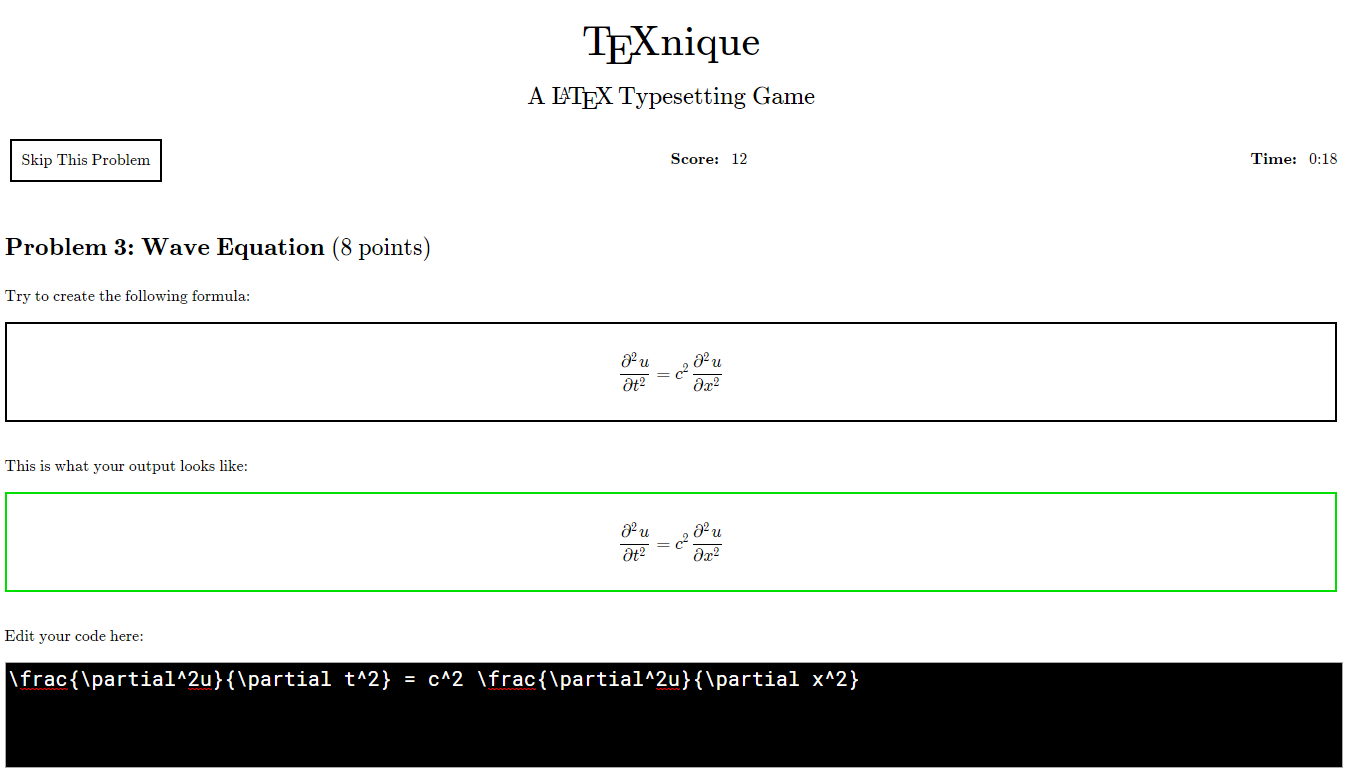
\includegraphics[width=1.0\linewidth,frame=]{./graphics/texnique.png}

% Caption is defined with a short and long version. The short version is shown in the 
% List of Figures section, and the long version is used directly with the figure. 			
	\caption[A screenshot of TeXnique, a game about typesetting equations.]{TeXnique, a game about typesetting equations \cite{texnique}. (Top) The game presents you with a rendered equation, (Bottom) the task is to enter LaTeX code that produces the same rendered equation. The green border on the lower rendering indicates it is a valid solution.}
	
% For figures label should be defined after the caption to ensure proper figure numbering.
	\label{fig:texnique}
\end{figure}
		
		TeXnique \cite{texnique} is web-browser based game for practising how to typeset equations in LaTeX. The game will present you with a rendered equation and your task is to type LaTeX code into the box below it such that your code produces the same (or closely matching / pixel equivalent) rendered equation. Figure \ref{fig:texnique} shows the game during play, the bottom rendered equation is bordered in green to indicate it is a valid match with the target. 

		% An example of how to center a passage of text, control local fontsize, 
		% and create a properly formatted and clickable URL.
		\begin{center}
		{\small \url{https://texnique.xyz}}
		\end{center}
		
		This is one of the more painful parts of typesetting a document, so it really takes a special kind of sadism to come up with such a game. Least to say, graduate students and researchers can be an odd bunch, and when we found this it was surprisingly addictive to compete over. 
		
		
		
	\section{Figures}
	\label{sec:typesetting_figures}
	
	In this template figures are numbered starting with the current chapter number followed by a figure number that resets to 1 each new chapter. As you can see below, the first figure is labelled Figure \ref{fig:dragon} because we are in Chapter \ref{chap:typesetting}.
	
	Figures in LaTeX are defined using a \lstinline|\begin{figure}...\end{figure}| environment and often immediately begin rendering in centre aligned mode by calling \lstinline|\centering|. Listing \ref{lst:latex_figure} below shows the LaTeX code used to typeset figure \ref{fig:dragon}. Figures \ref{fig:example_2x1} and \ref{fig:example_2x2} are defined similarly and make additional use of the \lstinline|\subfloat| command to position multiple images within a single figure environment, each with their own automatically incremented labels and individual captions.

	\lstinputlisting[label={lst:latex_figure}, caption={An example LaTeX excerpt demonstrating how to typeset figure \ref{fig:dragon} with a simple caption.}]{./listings/example_figure.tex}

	\subsection{Consistent presentation throughout the document}
		Figures work best in a document when you use a consistent style for formatting and captioning them and make sure that figures always actively support the content of the main text. 
	
	\subsection{Justified use of space in the document}
		All figures must be referred to directly in the main text of the document and discussed with meaningful and in depth critical analysis. If you don't need to use the figure to leverage and support your discussion then it is just taking up space and padding out the document. For example, you can use a command like \lstinline|\ref{fig:dragon}| to automatically get the figure number for Figure \ref{fig:dragon}. 	
		
		% [H] means put the figure HERE, directly when you input this code.
\begin{figure}[H]
	\centering

% We set the width of the figure based on the width of one line of text on the page. 
% The value can be tuned to any value in [0.0, 1.0] to scale the image while maintaining its aspect ratio.
	\includegraphics[width=1.0\linewidth]{./graphics/dragon.png}
	
% Caption is defined with a short and long version. The short version is shown in the 
% List of Figures section, and the long version is used directly with the figure. 		
	\caption[An image of many glass dragons being used to demonstrate typesetting a figure.]{A good caption should be sufficient enough to put the figure in context even if the reader has randomly flicked to the current page and looked only at the figure in isolation. All figures should also be referred to directly within the main text of your document. You can use the LaTeX \textbf{$\backslash$ref\{key\}} command to insert the correct figure number when you refer to it in the main text. By the very logic of this caption, this is a very poor caption because we still don't know why on earth is there an picture of glass dragons here. Image of glass dragons rendered using Path Tracing \cite{whittle15_dragons}.}
	
% For figures label should be defined after the caption to ensure proper figure numbering.
	\label{fig:dragon}
	
\end{figure}
		
	\subsection{Placement that supports and enhances the flow of the document}
		All figures shown in your document should be displayed in relevant locations, ideally just after that have been alluded to in the main text. Although there are many times where it is best to force a figure to the top or bottom of a nearby page.
	
	\subsection{Avoid directly importing other peoples images}
		You should avoid using other peoples figures whenever possible, and instead create your own figures for visualizing the specific methods and data you are working with in a way directly relevant to your project. 
	
	\subsection{Format sub-figures in LaTeX, not in the image itself}
		Construct sub-figures from multiple image files in LaTeX not in the image file itself. This allows you to tweak the positioning and layout without having to modify the images. It also allows for automatic formatting and numbering of captions and sub-captions. Figures \ref{fig:example_2x1} and \ref{fig:example_2x2} show examples of side-by-side and quad layouts respectively.
		
		% [H] means put the figure HERE, directly when you input this code.
\begin{figure}[H]
	\centering
	
% We use a figure width of 48.5% of the width of one line of text on 
% the page so there is some space between the images.
	\subfloat[Left image sub-caption.]{
		\includegraphics[width=0.485\linewidth]{./graphics/dragon.png}\label{fig:example_2x1_a}
	}~ % Use a tilde to add spacing for sub-figures that are displayed next to one another horizontally.
	\subfloat[Right image sub-caption.]{
		\includegraphics[width=0.485\linewidth]{./graphics/dragon.png}\label{fig:example_2x1_b}
	}\\ % New line before caption.

% Caption is defined with a short and long version. The short version is shown in the 
% List of Figures section, and the long version is used directly with the figure. 	
	\caption[A demonstration of a 2x1 sub-figure layout.]{Construct sub-figures from multiple image files in LaTeX not in the image file itself. This allows you to tweak the positioning and layout without having to modify the images. It also allows for automatic formatting and numbering of captions and sub-captions. Image of glass dragons rendered using Path Tracing \cite{whittle15_dragons}.}
	
% For figures label should be defined after the caption to ensure proper figure numbering.
	\label{fig:example_2x1}
	
\end{figure}
		
		% [H] means put the figure HERE, directly when you input this code.
\begin{figure}[H]
	\centering
	
% We use a figure width of 48.5% of the width of one line of text on 
% the page so there is some space between the images.
	\subfloat[Top-Left image sub-caption.]{
		\includegraphics[width=0.485\linewidth]{./graphics/dragon.png}\label{fig:example_2x2_a}
	}~ % Use a tilde to add spacing for sub-figures that are displayed next to one another horizontally.
	\subfloat[Top-Right image sub-caption.]{
		\includegraphics[width=0.485\linewidth]{./graphics/dragon.png}\label{fig:example_2x2_b}
	}\\ % New line before caption.
	\subfloat[Bottom-Left image sub-caption.]{
		\includegraphics[width=0.485\linewidth]{./graphics/dragon.png}\label{fig:example_2x2_c}
	}~ % Use a tilde to add spacing for sub-figures that are displayed next to one another horizontally.
	\subfloat[Bottom-Right image sub-caption.]{
		\includegraphics[width=0.485\linewidth]{./graphics/dragon.png}\label{fig:example_2x2_d}
	}\\ % New line before caption.
		
% Caption is defined with a short and long version. The short version is shown in the 
% List of Figures section, and the long version is used directly with the figure. 	
	\caption[A demonstration of a 2x2 sub-figure layout.]{A demonstration of a 2x2 sub-figure layout. Between A-B and C-D we use tilde symbols and between B-C we use a new line. Image of glass dragons rendered using Path Tracing \cite{whittle15_dragons}.}
	
% For figures label should be defined after the caption to ensure proper figure numbering.
	\label{fig:example_2x2}
	
\end{figure}
	
	\subsection{Robust captions that can stand in isolation}
		Figures need to be captioned such that they can be viewed in isolation and still be meaningful to the viewer. There will likely be some duplication of information that is written in the main text, but this is intended. 
	
	\subsection{Proper attribution and citation of images}
		\label{sec:typesetting_figures_citation}
		
		If an image does not belong to you it \textbf{must} be cited directly in the figure caption. \textbf{It is not correct to put a URL in the figure caption directly.} A URL in isolation is not an accurate or reliable way of directing a future reader to the exact content you are referencing. Instead make a new entry in your \lstinline|citations.bib| file and then reference that citation in the caption using the \lstinline|\cite{key}| command. Figures \ref{fig:dragon}, \ref{fig:example_2x1}, and \ref{fig:example_2x2} each include a statement in the caption stating ``Image of glass dragons rendered using Path Tracing \cite{whittle15_dragons}.''. When adding the BibTeX entry, try to find the proper information about the original author and source document to strengthen the citation in case the URL changes. 
	
	\section{Code Listings}
	\label{sec:typesetting_listings}
	
	Code listings should be formatted in the same style as figures and inline equations. It is important to use a monospace font so that characters line up vertically. Syntax highlighting is also extremely important for effectively displaying complicated code segments. To format inline code listings you can use the \lstinline[mathescape]|\lstinline$|$the_code$|$| command\footnote{So meta.}.
	
	% Longform Code listings should live in a code file, not embedded directly into your LaTeX code!
	\lstinputlisting[language={c}, label={lst:c_hello_world}, caption={An implementation of an important algorithm from our work.}]{./listings/hello_world.c}
	
	In LaTeX the ``Listings'' package can be used to properly format code and provide basic syntax highlighting, line numbering, and captioning of embedded code excerpts. Listing \ref{lst:listings} shows examples of how to properly format code using the listings package. 
	
	\newpage
	
	% Longform Code listings should live in a code file, not embedded directly into your LaTeX code!
	\lstinputlisting[label={lst:listings}, caption={Examples of methods for typesetting code listings within a LaTeX document.}]{./listings/listings.tex}
	
	\section{Tables}
	\label{sec:typesetting_tables}
	
	Tables are also quite predictably captioned and formatted the same way. It is important to decide on a style for how you will organize your data and apply that style consistently for all of your tables. Table \ref{tbl:example_table} shows one possible way of styling your data but is by no means the only way of doing so neatly. Consistency is the key. 
	
	% It's often a good idea to generate the LaTeX code for tables (python script or similar) so that if you rerun your code you don't have to typeset your results again by hand!
\begin{table}[H]
	\centering
	\scriptsize
	\caption[A demonstration of a table typeset in LaTeX.]{An example of a table formatted with caption.}
	
	% Tune the following two values that are being multiplied by the variable \textwidth
	% to control how large the scale of the table is, and how much is is squashed back 
	% to the final size.	
	\resizebox{0.8\textwidth}{!}{
		\begin{tabularx}{0.46\textwidth}{c|c|c|c|c|c}
			\toprule
			Some & Relevant & Fields & From & Your & Data\\
			\midrule
			0 & 0 & 0 & 0 & 0 & 0\\
			1 & 1 & 1 & 1 & 1 & 1\\
			2 & 2 & 2 & 2 & 2 & 2\\
			\bottomrule
		\end{tabularx}
		\label{tbl:example_table}
	}
\end{table}




	
